\documentclass[12pt, titlepage]{article}
% naglowek i stopka
\usepackage{fancyhdr}
% polskie znaki
\usepackage[utf8]{inputenc}
\usepackage[polish]{babel}
\usepackage{polski}
% czcionka Times
\usepackage[T1]{fontenc}
\usepackage{mathptmx}
% ------------------
% marginesy
\usepackage{geometry} 
\newgeometry{tmargin=3cm, bmargin=3cm, lmargin=2cm, rmargin=2cm}
% przedefiniowanie kolumn w tabelach
% mozna ustawiac im szerokosc
\usepackage{array}
\newcolumntype{L}[1]{>{\raggedright\let\newline\\\arraybackslash\hspace{0pt}}m{#1}}
\newcolumntype{C}[1]{>{\centering\let\newline\\\arraybackslash\hspace{0pt}}m{#1}}
\newcolumntype{R}[1]{>{\raggedleft\let\newline\\\arraybackslash\hspace{0pt}}m{#1}} 
% ------------------------------
% napisy nad tabelami
\usepackage[font=small,format=plain,up,textfont=normal,up,justification=justified,singlelinecheck=false]{caption}
% tabele na kilka stron
\usepackage{longtable}
% ustawienie tabeli w miejscu
\usepackage{float}
% spis tresci z linkami do sekcji
\usepackage{hyperref}
\hypersetup{
	colorlinks,
	citecolor=black,
	filecolor=black,
	linkcolor=black,
	urlcolor=blue
}
% kolowanie tabeli
%\usepackage[table]{xcolor}
\usepackage{color, colortbl}
% dodawanie obrazkow
\usepackage{graphicx}

\fancypagestyle{firstpage}{					% strona tytulowa
	\renewcommand{\headrulewidth}{0pt}
	\renewcommand{\footrulewidth}{0.4pt}
	\fancyhf{}% clear all fields
	\fancyfoot[C]{Poznań, \today}%
	\fancyhead[C]
		{
		POLITECHNIKA POZNAŃSKA\\
		WYDZIAŁ ELEKTRYCZNY, INFORMATYKA\\
		SEMESTR VI, GRUPA BSI-2
		}
}

\fancypagestyle{plain}{						% zwykla strona
	\renewcommand{\headrulewidth}{0pt}%
	\fancyhf{}% clear all fields
	\fancyfoot[R]{\thepage}%
}
\pagestyle{plain}


\begin{document}
	\begin{titlepage}
		\thispagestyle{firstpage}
		\centering
			\vspace*{5cm}
			{\huge Podstawy Teleinformatyki\\
				WebScrapper / Metawyszukiwarka\\}
			\vspace{6cm}
			{\large \url{}\\}
			\vspace{1cm}
			{\large
			Paweł Soja\\
			Numer indeksu: 122031\\
			pawel.soja@student.put.poznan.pl\\
			\vspace{0.5cm}
			Krzysztof Łuczak\\
			Numer indeksu: 122008\\
			krzysztof.t.luczak@student.put.poznan.pl\\
			\vspace{0.5cm}
			Dawid Wiktorski\\
			Numer indeksu: 122056\\
			dawid.wiktorski@student.put.poznan.pl\\}
	\end{titlepage}
	\tableofcontents
	\listoftables
	
	\newpage
	\section{Opis i uzasadnienie wyboru tematu}
	Celem projektu jest zbudowanie platformy do zbierania i prezentowania danych z różnych stron internetowych. Platforma składa się z serwisu internetowego prezentującego dane użytkownikom zalogowanym oraz z aplikacji zbierających te dane.
	
	Na potrzeby tego projektu i dokumentacji utworzone zostało pojęcie 'scrapowanie', które oznaczać będzie zbieranie danych ze stron internetowych poprzez odwiedzenie jej i zapisanie wybranych informacji do bazy danych.
	
	\subsection{Ogólny proces zbierania i przetwarzania danych}
	Informacje zbierane są przez tzw. scrapery, a następnie zapisywane w bazie danych. Scraper zbiera tylko te dane, które zostaną ustalone przez programistę. Dalsze filtrowanie odbywa się na poziomie aplikacji internetowej w oparciu o profil użytkownika lub podane parametry. Wyszukiwanie wykonywane jest w bazie danych. Dane zapisywane w bazie usuwane są po ustalonym czasie. Dlatego też aplikacja umożliwia filtrowanie wstecz, ale tylko do pewnej granicy. Dane zapisane w bazie można określić jako 'newsy'. Jeżeli informacja zostaje usunięta to znaczy, że jest już nieaktualna. Dzięki takiemu systemowi gromadzenia danych, aplikacja jest w stanie serwować użytkownikom najnowsze materiały, przy jednoczesnym zachowaniu wydajności filtrowania różnych źródeł. Z założenia użytkownik regularnie korzysta z aplikacji.
	
	\subsection{Uzasadnienie wyboru tematu}
	Temat wybraliśmy, ponieważ interesuje nas dziedzina przetwarzania danych. Chcielibyśmy poznać technologie scrapowania, parsowania stron internetowych oraz język Python, framework Django i technologie front-endowe tj. HTML5, Javascript. Jednocześnie nie znaleźliśmy zadowalającego nas serwisu, który udostępniałby takie usługi, dlatego sami zdecydowaliśmy zrobić swój.
	
	\newpage
	\section{Organizacja pracy}
	Przy pracy nad projektem, korzystano z repozytorium GitHub. Link do repozytorium: \newline
	\textcolor{blue}{\href{https://github.com/vizarch/projektPT}{WebSrapper/Metawyszukiwarka}}
	\subsection{Harmonogram prac}
	Orientacyjny harmonogram prac został przedstawiony w tablicy 1. Wyszczególniono zadania oraz osobę/osoby zajmujące się danym fragmentem projektu.
	\definecolor{azure3}{rgb}{0.0, 0.7, 1.0}
	\begin{table}[H]
		\setlength\extrarowheight{5pt}
		\centering
		\caption{Harmonogram prac}
		\label{harmonogram_prac}
		\begin{tabular}{ | C{2cm} | C{8cm} | C{6cm} | }
			\hline
			\rowcolor{azure3}
			\textbf{Lp.} &	\textbf{Opis} &	\textbf{Miesiąc} \\ \hline

			1.& Wybór technologii, modułów, podział pracy & Marzec \\ \hline

			2.&	Wstępna dokumentacja, planowanie serwisu &	Kwiecień \\ \hline

			3.&	Zapoznanie z technologią, testy bibliotek &	Kwiecień \\ \hline

			4.&	Baza danych, pierwszy moduł, interfejs & Maj \\ \hline

			5.&	Kolejne moduły & Maj \\ \hline

			6.&	Testowanie serwisu, poprawki &	Czerwiec \\ \hline

			7.&	Zakończenie prac nad serwisem &	Czerwiec \\ \hline

		\end{tabular}
	\end{table}
	
	\subsection{Podział prac pomiędzy członków zespołu}
	W tablicy 2 przedstawiono podział prac pomiędzy członków zespołu.
	\definecolor{azure}{rgb}{0.0, 0.4, 1.0}
	\definecolor{azure2}{rgb}{0.94, 1.0, 1.0}
	\definecolor{azure3}{rgb}{0.0, 0.7, 1.0}
	\begin{table}[H]
		\setlength\extrarowheight{5pt}
		\centering
		\caption{Podział prac}
		\label{podzial_prac}
		\begin{tabular}{ | C{2cm} | C{6cm} | C{8cm} | }
			\hline
			\rowcolor{azure3}
			\textbf{Lp.} &	\textbf{Opis} &	\textbf{Osoby} \\ \hline
			%\rowcolor{azure2}
			1.	&	Baza danych			&	Wszyscy \\ \hline
			%\rowcolor{azure3}
			2.	&	Projekt interfejsu	&	Paweł Soja \\ \hline
			%\rowcolor{azure2}
			3.	&	Front-end serwisu	&	Paweł Soja \\ \hline
			%\rowcolor{azure3}
			4.	&	Back-end serwisu	&	Krzysztof Łuczak, Dawid Wiktorski \\ \hline
			%\rowcolor{azure2}
			5.	&	Moduł I				&	Krzysztof Łuczak \\ \hline
			%\rowcolor{azure3}
			6.	&	Moduł II			&	Dawid Wiktorski \\ \hline
			%\rowcolor{azure2}
			7.	&	Moduł III			&	Dawid Wiktorski \\ \hline
				%\rowcolor{azure2}
			8.	&	Moduł IV			&	Dawid Wiktorski \\ \hline
				%\rowcolor{azure2}
			9.	&	Moduł V			&	Dawid Wiktorski \\ \hline
			%\rowcolor{azure3}
			10.	&	Testowanie			&	Wszyscy \\ \hline
			%\rowcolor{azure2}
		\end{tabular}
	\end{table}

	\subsection{Środowisko pracy}
	\begin{itemize}
		\item IDE PyCharm,
		\item TeXstudio,
		\item przeglądarki internetowe: Google Chrome oraz Mozilla Firefox.
	\end{itemize}
	\newpage
	\section{Wymagania}
	\subsection{Opis funkcjonalności}
	{\large Aktorzy systemu:
	\begin{itemize}
		\item użytkownik
			\begin{itemize}
				\item użytkownik zalogowany - posiada prawa do użytkowania serwisu,
				\item użytkownik niezalogowany - może dokonać rejestracji,
				\item administrator - zarządza serwisem,
			\end{itemize}
		\item aplikacja internetowa - prezentuje dane,
		\item moduł zbierający dane (scraper) - zbiera i przetwarza dane. \newline
	\end{itemize}}

	 Wymagania funkcjonalne systemu scharakteryzowano w tablicy 3. 
	\definecolor{azure3}{rgb}{0.0, 0.7, 1.0}
	\setlength\extrarowheight{10pt}
	\begin{longtable}{ | C{5cm} | C{8cm} | C{4.5cm} |}
		\caption{Funkcjonalności}
		\label{funkcjonalnosci}
		\endfirsthead % musi byc
		\multicolumn{3}{l}%
		{\tablename\ \thetable\ -- \textit{Kontynuacja}}\hfill  \\
		\hline
		\rowcolor{azure3}
		\textbf{Funkcja} & \textbf{Opis} & \textbf{Aktorzy} \\
		\hline
		\endhead
		\hline
		\rowcolor{azure3}
		\textbf{Funkcja} & \textbf{Opis} & \textbf{Aktorzy} \\
		\hline
		Przeglądanie strony głównej	&	
		Możliwość przeglądania strony głównej serwisu. &
		Użytkownicy \\ 
		\hline
		Rejestracja &
		Możliwość zarejestrowania konta w serwisie. &
		Użytkownik niezalogowany \\
		\hline
		Potwierdzenie rejestracji, zmiany hasła lub zmiany adresu e-mail konta&
		Możliwość potwierdzenia rejestracji, zmiany hasła lub zmiany adresu e-mail konta poprzez kliknięcie link aktywacyjny wysłany pocztą elektroniczną.&
		Użytkownik niezalogowany \\
		\hline
		Logowanie &
		Możliwość logowania się do serwisu.&
		Użytkownik niezalogowany \\
		\hline
		Wylogowanie & Możliwość wylogowania się z serwisu. &
		Użytkownik zalogowany, administrator \\
		\hline
		Zmiana hasła do konta &
		Możliwość zmiany hasła do aktywnego konta.&
		Użytkownik zalogowany, administrator \\
		\hline
		Zmiana adresu e-mail konta &
		Możliwość zmiany adresu e-mail konta. &
		Użytkownik zalogowany, administrator \\
		\hline
		Ustawienie profilu źródeł &
		Możliwość wybrania źródeł, z których otrzymywane będą informacje. &
		Użytkownik zalogowany, administrator \\
		\hline
		Ustawienie profilu tagów &
		Możliwość wybrania tagów, na podstawie których filtrowane będą informacje. &
		Użytkownik zalogowany, administrator \\
		\hline
		Ustawienie filtra daty &
		Możliwość wybrania przedziału czasowego, na podstawie którego filtrowane będą informacje. &
		Użytkownik zalogowany, administrator \\
		\hline
		Zbieranie danych ze strony i parsowanie ich &
		Scraper zbiera dane ze strony, parsuje je oraz zapisuje do bazy danych. Jeden scraper zbiera dane z jednej strony. &
		Scraper \\
		\hline
	\end{longtable}

	\subsection{Wymagania pozafunkcjonalne}
		\begin{itemize}
		\item zainstalowany interpreter języka Python w wersji 3.5 lub wyższej,
		\item zainstalowana biblioteka "BeautifulSoup",
		\item język interfejsu użytkownika: polski,
		\item bezpieczne przechowywanie haseł w formie zahaszowanej.
		\newline
		\end{itemize}

	\newpage
	\section{Wybrane technologie i uzasadnienie}
	\begin{itemize}
		\item Back-end - \texttt{Python, Django}
		\begin{itemize}
			\item stosunkowo krótki czas tworzenia aplikacji przy jednoczesnym zachowaniu: \begin{itemize}
				\item pełnej funkcjonalości,
				\item stabilności,
				\item wydajności	
			\end{itemize}
		\end{itemize}
		\item Front-end - \texttt{HTML5, Javascript}
		\begin{itemize}
			\item uniwersalna technologia, która jest wspierana przez wszystkie popularne przeglądarki internetowe
		\end{itemize}
		\item Baza danych - \texttt{SQLite}
		\begin{itemize}
			\item prosta integracja z językiem Python,
			\item dobra we wstępnej fazie projektu
		\end{itemize}
	\end{itemize}
	
	\subsection{Biblioteka BeautifulSoup}
	Bibliotek do wyciągania danych ze stron internetowych jest wiele, są to między innymi: \texttt{ Scrapy},\texttt{ BeautifulSoup}, \texttt{Urllib2},\texttt{ MarkupSafe} oraz \texttt{feedparser}. W projekcie wykorzystaliśmy bibliotekę BeautifulSoup, która przeznaczona jest dla języka Python. Umożliwia ona wyciąganie danych z plików HTML oraz XML. BeautifulSoup w wersji 4 współracuje z takimi parserami jak:\texttt{ Python html.parser},\texttt{ lxml HTML parser}, \texttt{lxml XML parser} i \texttt{htm5lib}. Po przeprowadzonych testach, lxml HTML parser okazał się najszybszym oraz najbardziej niezawodym parserem spośród wyżej wymienionych. Dużą zaletą biblioteki BeautifulSoup jest łatwa implemetacja w architekturze modułowej.

	\newpage
	\section{Architektura rozwiązania}
	W projekcie została wykorzystana relacyjna baza danych SQLite. Na rysunku 1 przedstawiono schemat relayjny bazy danych. 
		\begin{figure}[H]
			\centering
			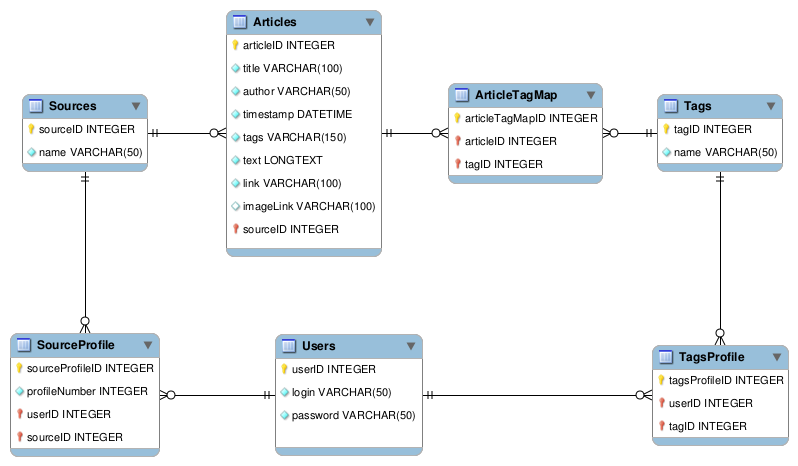
\includegraphics[scale=0.68]{obrazki/schemat_bd.png}
			\caption{Schemat bazy danych}
			\label{fig:db_schema}
		\end{figure}
	W tablicy 4 scharakteryzowano bazę danych.
	\definecolor{azure3}{rgb}{0.0, 0.7, 1.0}
	\setlength\extrarowheight{10pt}
	\begin{longtable}{ | C{5cm} | C{12cm} |}
		\caption{Opis bazy danych}
		\label{opis_bazy_danych}
		\endfirsthead % musi byc
		\multicolumn{2}{l}%
		{\tablename\ \thetable\ -- \textit{Kontynuacja}}\hfill  \\
		\hline
		\rowcolor{azure3}
		\textbf{Tabela} & \textbf{Opis} \\
		\hline
		\endhead
		\hline
		\rowcolor{azure3}
		\textbf{Tabela} & \textbf{Opis} \\
		\hline	
		Articles &
		Zawiera wszystkie sparsowane strony. \\ 
		\hline
		Tags &
		Zawiera wszystkie dostępne tagi. Dodanie nowego taga odbywa się automatycznie, gdy scraper podczas parsowania wykryje, że danego taga jeszcze nie ma w bazie. \\
		\hline
		ArticleTagMap &
		Łączy daną stronę z odpowiednim tagiem. \\
		\hline
		Sources &
		Zawiera wszystkie dostępne źródła, czyli strony internetowe, z których zbieramy dane. Dodanie odbywa się ręcznie. Administrator musi napisać moduł dla danej strony. \\
		\hline
		Users &
		Zawiera wszystkich użytkowników serwisu. \\
		\hline
		TagsProfile &
		Łączy użytkownika z tagami, które wybrał. \\
		\hline
		SourceProfile &
		Łączy użytkownika z źródłami danych, które wybrał. \\
		\hline
	\end{longtable}
	\newpage
	\section{Interesujące problemy i ich rozwiązania}
	Podczas implementacji modułów, w każdym z nich, spotkano się z problemem wyciągania potrzebnych danych ze stron internetowych. Przy parsowaniu stron, najczęściej nieznajdywanym elementem w artykule okazał się link do obrazka. Rozwiązaniem problemu było najpierw ustawienie domyślego obrazka dla danego modułu oraz wykorzystanie go, gdy parser nie poradził sobie ze znalezieniem obrazka w artykule.   
		\subsection{Moduł scrapujący sekurak.pl}
			Serwis sekurak.pl zawiera dwa rodzaje artykułów, które pobieramy. Pierwszy rodzaj znajduje się w kategorii "teksty", a drugi "w biegu". Scraper został podzielony na dwa wątki, każdy dla jednej z tych kategorii. To spowodowało przyspieszenie procesu zbierania o około 50\%. Algorytm sekwencyjny dla jednej strony artykułów wykonywał się około 24 s. Algorytm wielowątkowy około 14 s.
		\subsection{Moduł scrapujący altcontroldelete.pl}
			W serwisie altcontroldelete.pl data publikacji artykułu może być podana w języku polskim lub angielskim. Rozwiązaniem problemu było utworzenie dwóch słowników, które w odpowiedni sposób zinterpretują podaną datę. 
	\newpage
	\section{Opis stron internetowych, z których zbierane są informacje}
	Strony internetowe, z których zbierane są dane to:
	\begin{itemize}
	\item \url{www.sekurak.pl},
	\item \url{www.dobreprogramy.pl/Blog.html}
	\item \url{www.niebezpiecznik.pl}
	\item \url{www.pclab.pl/news.html}
	\item \url{www.altcontroldelete.pl}
	\end{itemize}  
	Poniżej w podrozdziałach przedstawiono dane, które są zbierane z każdej ze stron internetowych.
		\subsection{sekurak.pl}
		W tablicy 5 pokazano dane, które są zbierane ze strony sekurak.pl
		\begin{table}[H]
			\centering
			\caption{Parametry artykułów - sekurak.pl}
			\label{sekurak_parametry}
			\begin{tabular}{ | C{2cm} | C{4cm} | C{2cm} | C{2cm} | C{3cm} | C{2cm} | @{}m{0pt}@{}}
				\hline
				Tytuł & Data opublikowania & Tagi & Obrazek & Fragment tekstu & Link &\\[0.5cm]
				\hline
			\end{tabular}
		\end{table}

		\subsection{dobreprogramy.pl/Blog.html} 
		W tablicy 6 pokazano dane, które są zbierane ze strony dobreprogramy.pl/Blog.html
		\begin{table}[H]
			\centering
			\caption{Parametry artykułów - dobreprogramy.pl}
			\label{dobreprogramy_parametry}
			\begin{tabular}{ | C{2cm} | C{4cm} | C{2cm} | C{2cm} | C{3cm} | C{2cm} | @{}m{0pt}@{}}
				\hline
				Tytuł & Data opublikowania & Tagi & Autor & Fragment tekstu & Link &\\[0.5cm]
				\hline
			\end{tabular}
		\end{table}
		\subsection{niebezpiecznik.pl}
		W tablicy 7 pokazano dane, które są zbierane ze strony niebezpiecznik.pl
		\begin{table}[H]
			\centering
			\caption{Parametry artykułów - niebezpiecznik.pl}
			\label{niebezpiecznik_parametry}
			\begin{tabular}{ | C{1.5cm} | C{4cm} | C{1.5cm} | C{1.5cm} | C{1.5cm} | C{3cm} | C{1.5cm} | @{}m{0pt}@{}}
				\hline
				Tytuł & Data opublikowania & Tagi & Autor & Obrazek & Fragment tekstu & Link &\\[0.5cm]
				\hline
			\end{tabular}
		\end{table}
		\subsection{pclab.pl/news.html} 
		W tablicy 8 pokazano dane, które są zbierane ze strony pclab.pl/news.html
		\begin{table}[H]
			\centering
			\caption{Parametry artykułów - pclab.pl/news.html}
			\label{z3s_parametry}
			\begin{tabular}{ | C{1.5cm} | C{4cm} | C{1.5cm} | C{1.5cm} | C{1.5cm} | C{3cm} | C{1.5cm} | @{}m{0pt}@{}}
				\hline
				Tytuł & Data opublikowania & Tagi & Autor & Obrazek & Fragment tekstu & Link &\\[0.5cm]
				\hline
			\end{tabular}
		\end{table}
		\subsection{altcontroldelete.pl} 
		W tablicy 9 pokazano dane, które są zbierane ze strony altcontroldelete.pl
		\begin{table}[H]
			\centering
			\caption{Parametry artykułów - altcontroldelete.pl}
			\label{wykop_parametry}
			\begin{tabular}{ | C{1.5cm} | C{4cm} | C{1.5cm} | C{1.5cm} | C{1.5cm} | C{3cm} | C{1.5cm} | @{}m{0pt}@{}}
				\hline
				Tytuł & Data opublikowania & Tagi & Autor & Obrazek & Fragment tekstu & Link &\\[0.5cm]
				\hline
			\end{tabular}
		\end{table}
	
	\newpage
	\section{Instrukcja użytkowania aplikacji}
	W tym rozdziale przedstawiono interfejs strony internetowej wraz z instrukcją uzytkowania.
	\subsection{Strona główna}
	Po wejściu na stronę główną, użytkownikowi ukazuje się krótki opis funkcjonalności serwisu. Z tego miejsca użytkownik może przejść do kolejnej strony ze źródłami i tagami. Również ma możliwość zalogowania się lub założenia konta. Gdy, użytkownik poda złe dane w procesie logowania lub rejestracji, na stronie głównej pojawią się odpowiednie komunikaty. Na rysunku 2 ukazano stronę główną.
	\begin{figure}[H]
		\centering
		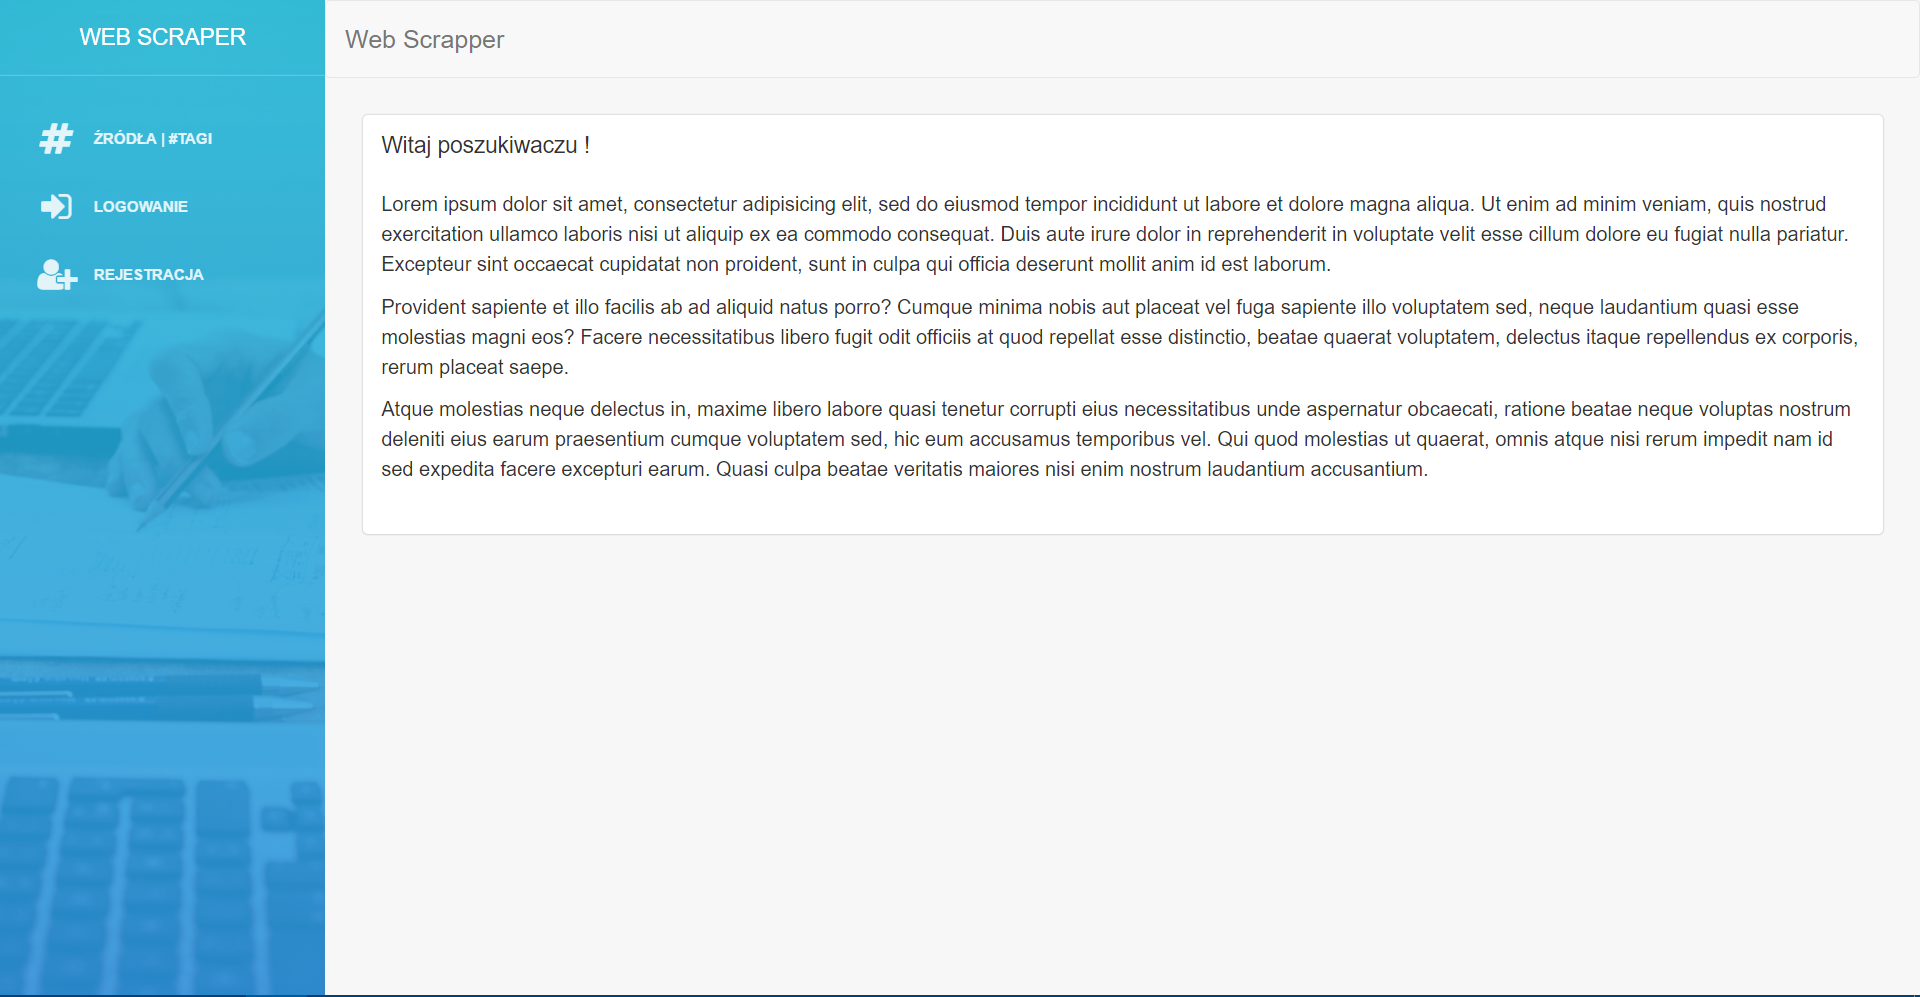
\includegraphics[scale=0.45]{obrazki/stronaGlowna.png}
		\caption{Strona główna}
		\label{fig:db_schema}
	\end{figure}

	\newpage
	\subsection{Źródła | \#Tagi dla użytkownika niezalogowanego}
	Na stronie związanej ze źródłami i tagami, użytkownik niezalogowany ma możliwość przejrzenia z jakich stron internetowych zbierane są dane. Przy każdym źródle pokazana jest liczba artykułów, które obecnie przechowywane są w bazie danych. Poniżej źródeł, wymienione są tagi, które również przechowywane są w bazie danych. Obok każdego z tagów występuje liczba, która wskazuje, ile jest artykułów związanych z danym tagiem. Na rysunku 3 ukazano stronę ze źródłami i tagami.
	\begin{figure}[H]
		\centering
		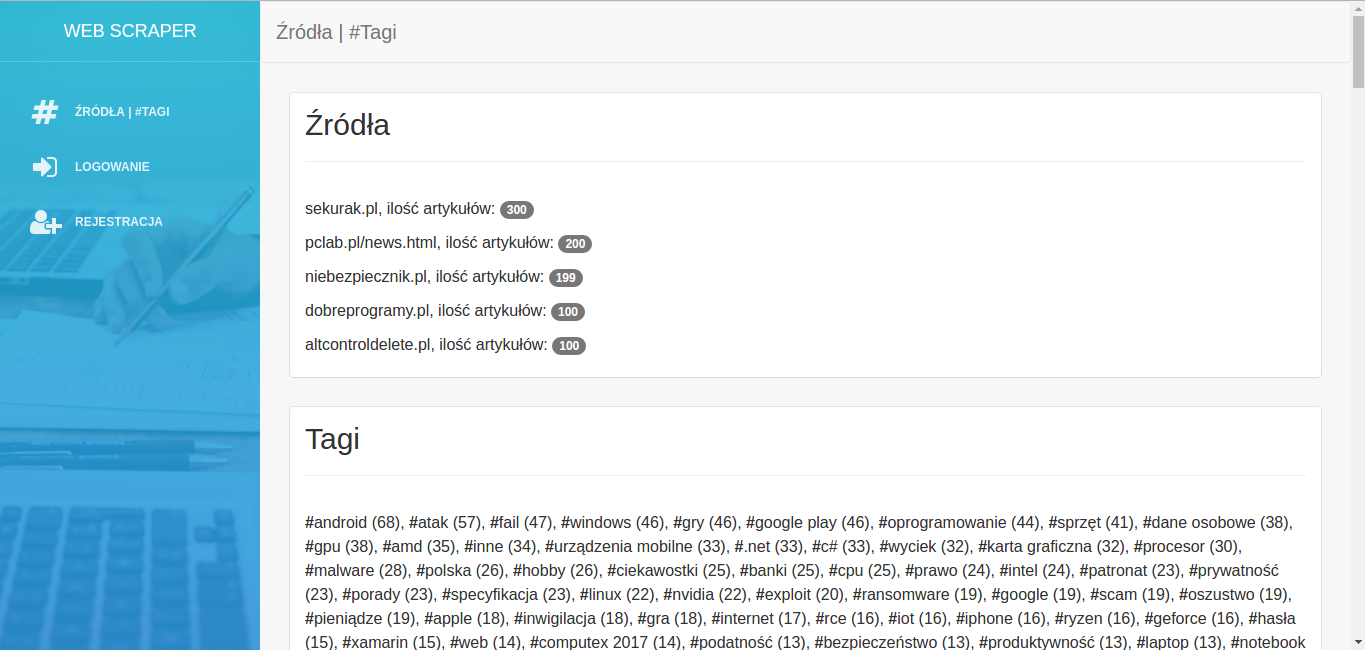
\includegraphics[scale=0.45]{obrazki/niezalogowanyZrodla.png}
		\caption{Źródła | \#Tagi dla użytkownika niezalogowanego}
		\label{fig:db_schema}
	\end{figure}
	
	\newpage
	\subsection{Wyszukiwarka}
\begin{figure}[H]
	\centering
	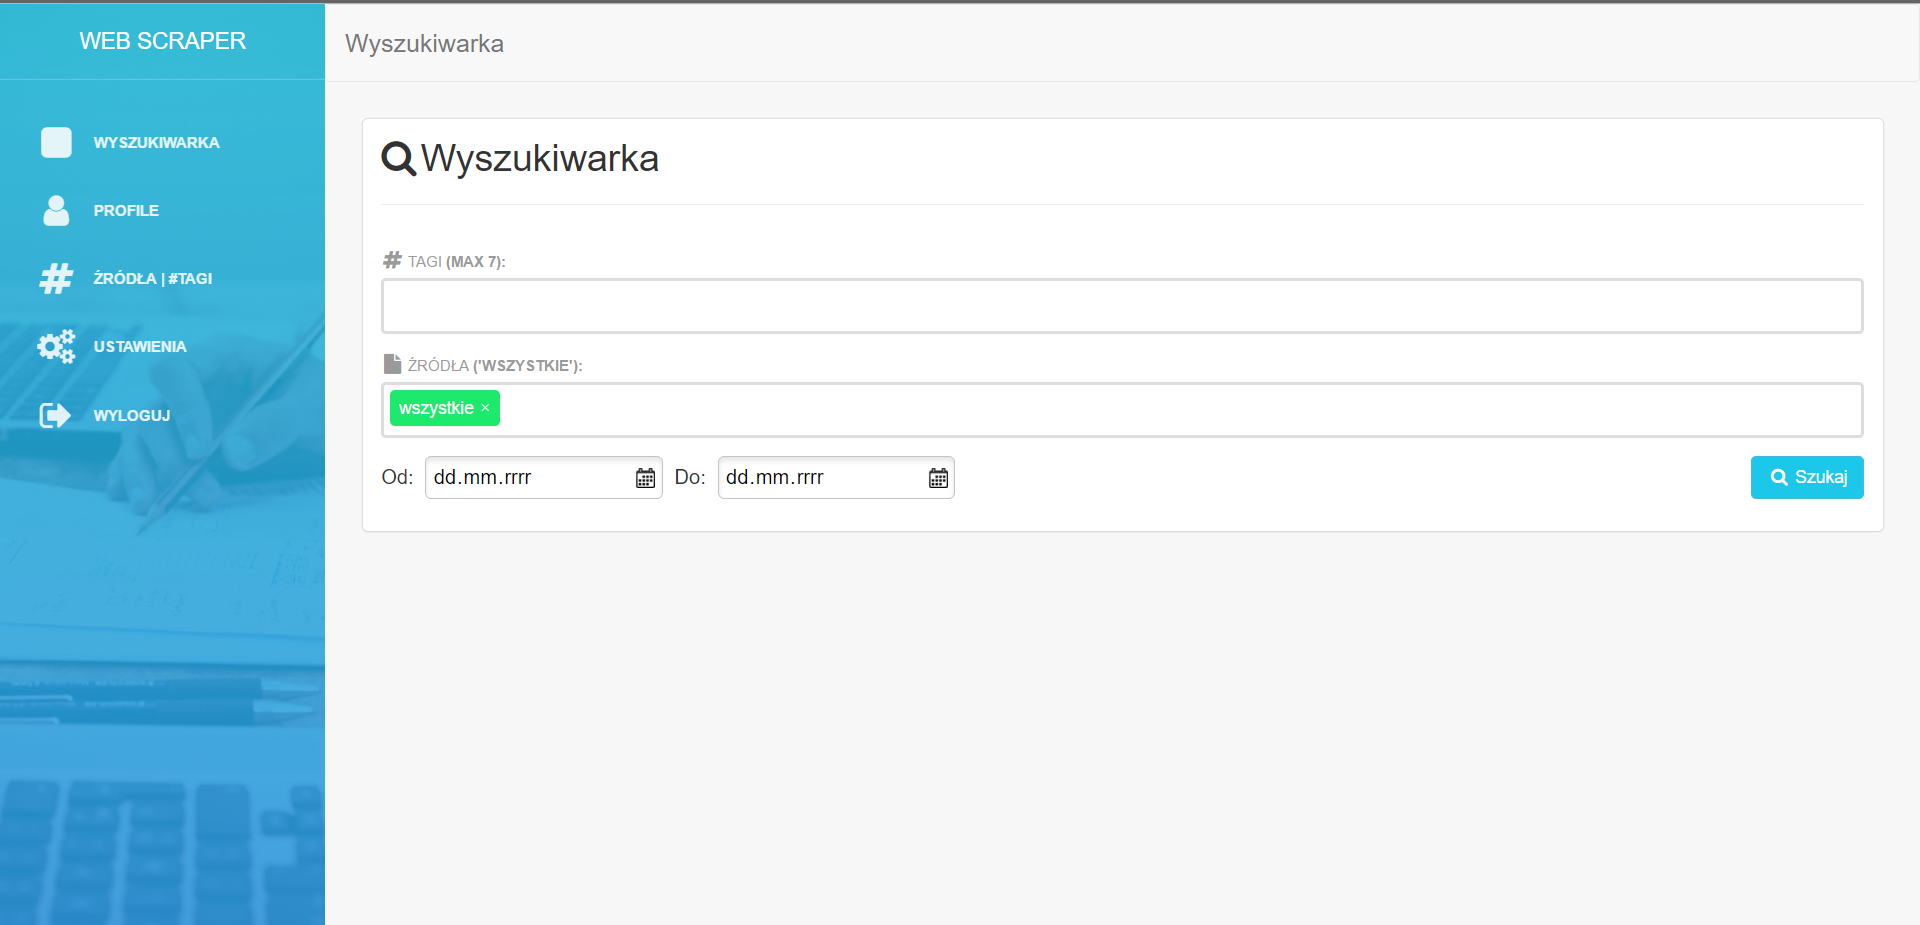
\includegraphics[scale=0.45]{obrazki/wyszukiwarka.png}
	\caption{Wyszukiwarka}
	\label{fig:db_schema}
\end{figure}


	\newpage
	\subsection{Profile}
	\begin{figure}[H]
	\centering
	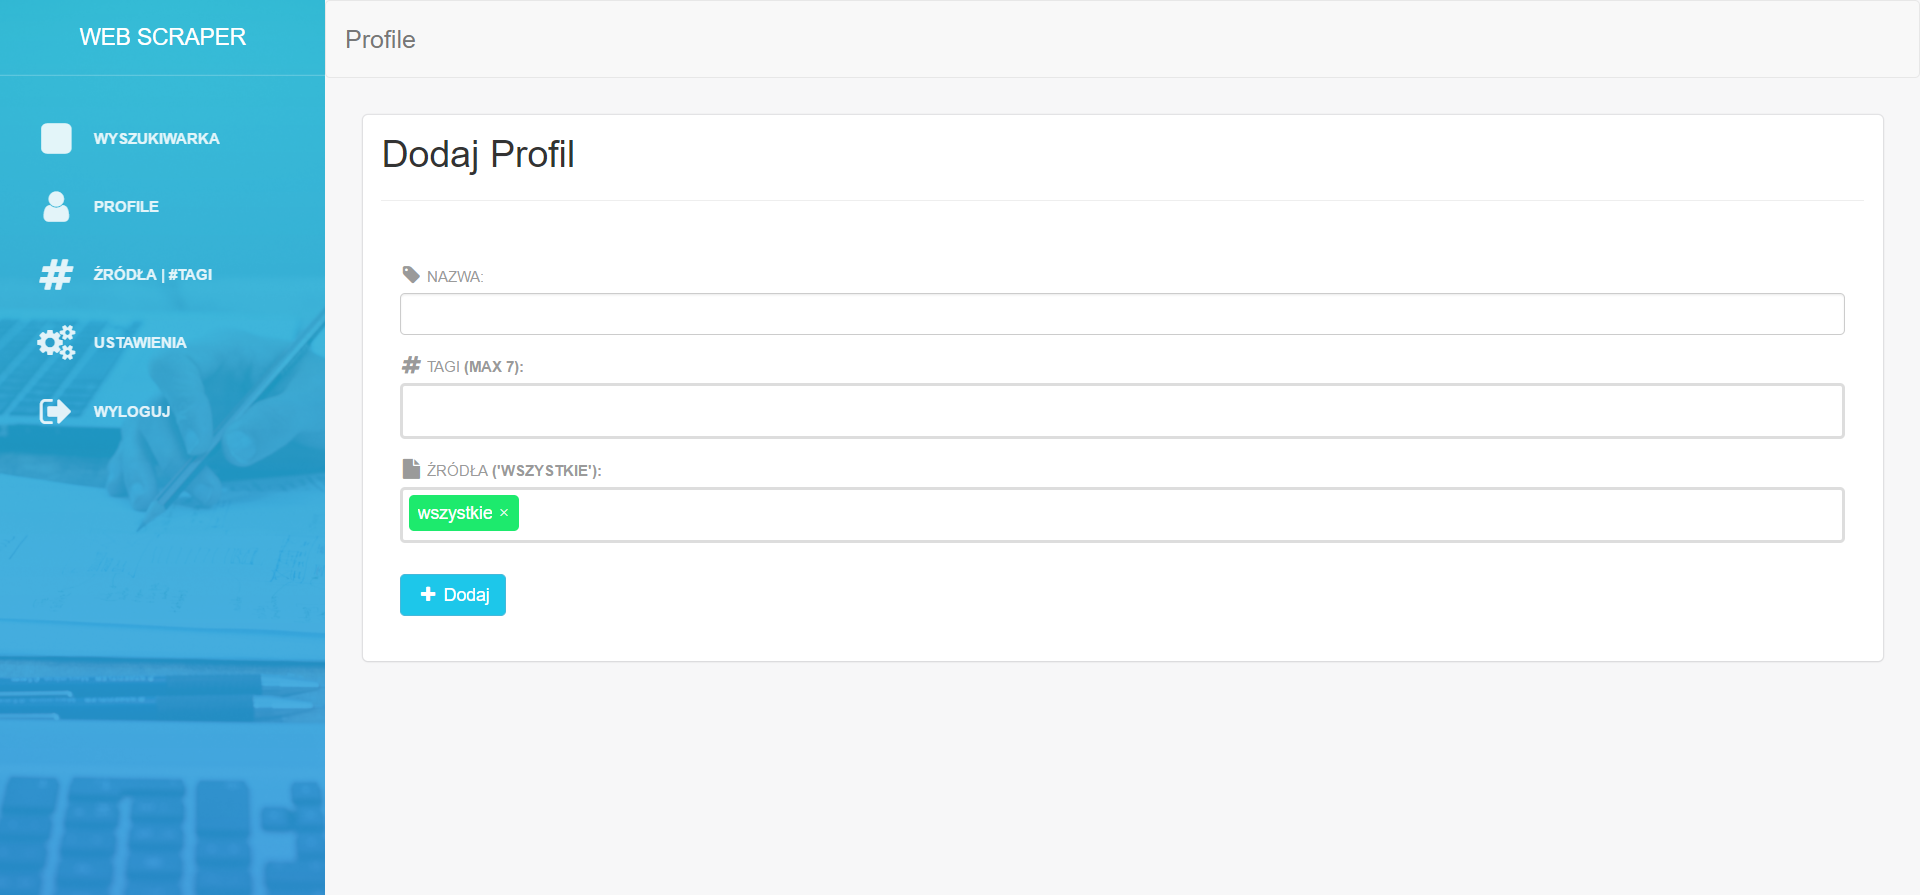
\includegraphics[scale=0.45]{obrazki/profile.png}
	\caption{Profile}
	\label{fig:db_schema}
	\end{figure}


	\newpage
	\subsection{Źródła | \#Tagi dla użytkownika zalogowanego}
	Użytkownik zalogowany na stronie ze źródłami i tagami ma możliwość nie tylko przejrzenia z jakich stron internetowych zbierane są dane i jakie tagi występują w bazie danych. Strona ta została rozszerzona o dodatkowe funkcjonalności. Użytkownik po kliknięciu na dany tag, otrzymuje listę powiązanych artykułów  z wybranym tagiem. Dodatkowo, po kliknięciu na dany artykuł, użytkownik przechodzi bezpośrednio do strony internetowej z artykułem. Na rysunku 6 ukazano stronę ze źródłami i tagami dla użytkownika zalogowanego, po wybraniu tagu \texttt{oprogramowanie}.
\begin{figure}[H]
	\centering
	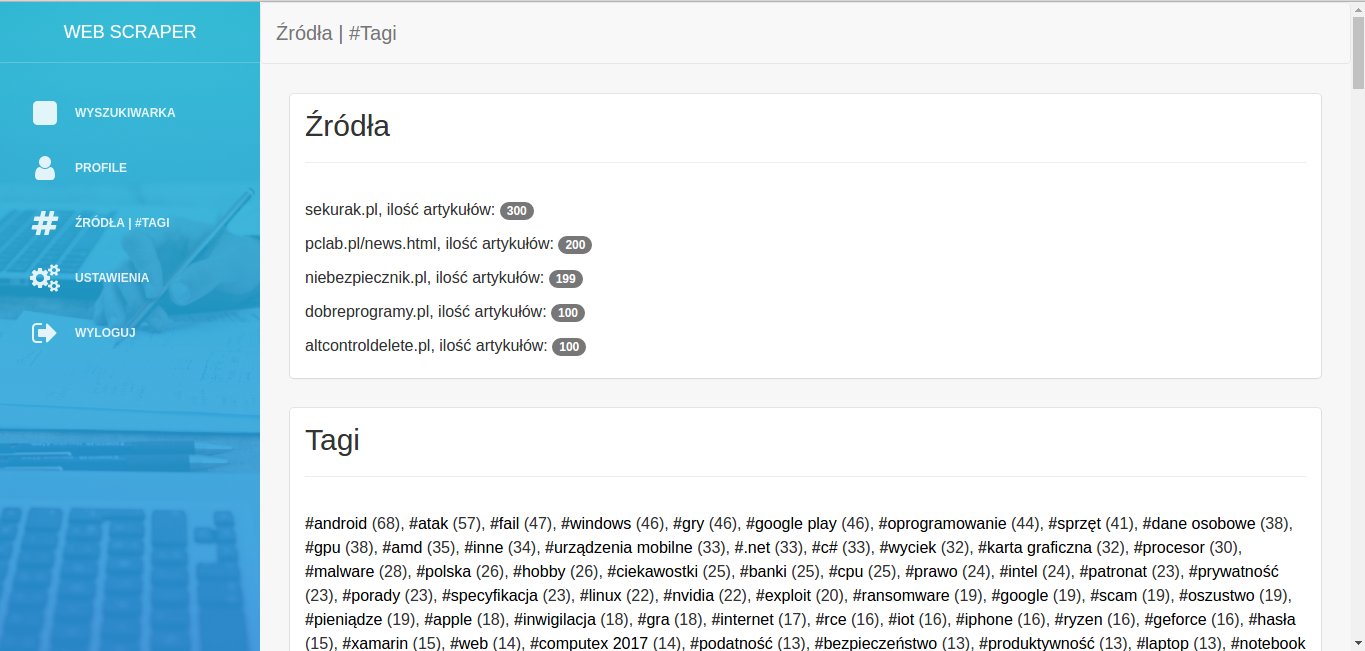
\includegraphics[scale=0.45]{obrazki/zalogowanyZrodla.png}
	\caption{Źródła | \#Tagi dla użytkownika zalogowanego}
	\label{fig:db_schema}
\end{figure}
	
	
	\newpage
	\subsection{Ustawienia}
	W ustawieniach, użytkownik ma możliwość zmiany hasła, zmiany adresu e-mail oraz usunięcia swojego konta. Na tej stronie, pojawią się również komunikaty związane z powyżej wymienonymi akcjami, które użytkownik jest w stanie zrobić. Gdy, użytkownik zmieni swój adres e-mail, automatycznie zostanie wylogowany i przekierowany do strony głównej. Na rysunku 7 ukazano stronę z ustawieniami.
	\begin{figure}[H]
		\centering
		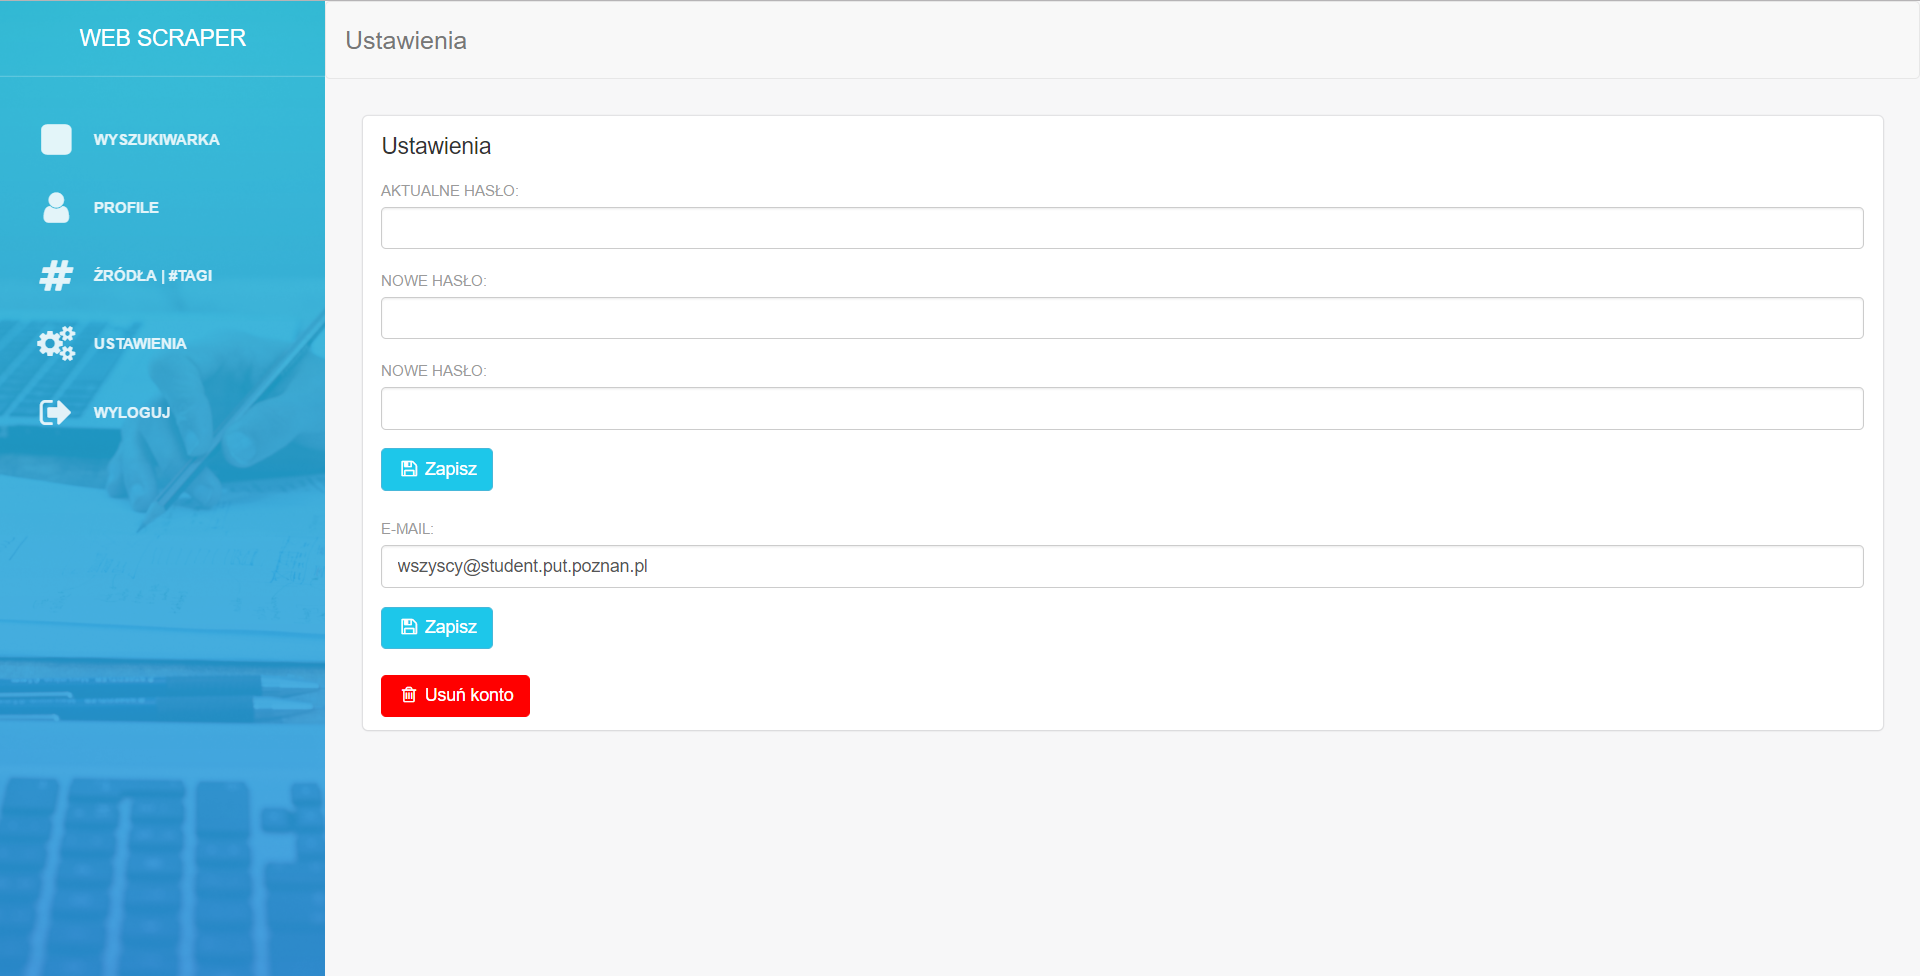
\includegraphics[scale=0.45]{obrazki/ustawienia.png}
		\caption{Ustawienia}
		\label{fig:db_schema}
	\end{figure}
	
\end{document}
